\documentclass[tikz,border=5mm]{standalone}
\begin{document}
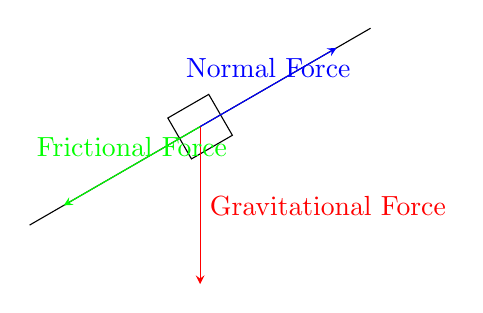
\begin{tikzpicture}

% Draw the inclined plane
\draw (0,0) -- (30:5cm);

% Draw the block
\node[minimum size=0.6cm,draw,rectangle,rotate=30] (B) at (30:2.5cm) {};

% center of mass
\coordinate (CoM) at (B.center);

% Draw the forces
\draw[-stealth,red] (CoM) -- ++(270:2cm) node[midway,right] {Gravitational Force};
\draw[-stealth,blue]  (CoM) -- ++(30:2cm) node[midway,above] {Normal Force};
\draw[-stealth,green] (CoM) -- ++(210:2cm) node[midway,above] {Frictional Force};

\end{tikzpicture}
\end{document}